\documentclass{book}

% Just to have them already
% \begin{sloppypar}
% \end{sloppypar}

% Just try to parse, do not ask for input
\nonstopmode

% Bibliography
% For Vancounter style:
\usepackage[numbers]{natbib}
% For regular style:
% \usepackage{natbib}


%\bibpunct{(}{)}{;}{a}{}{;}

% Use 'It was found that A is B (Name 1234)' style
%\setcitestyle{authoryear,open={},close={}}

% Affiliations
\title{
  Music
}
\author{Richèl J.C. Bilderbeek}


% Use double spacing
%\usepackage{setspace}
%\doublespacing

\usepackage{listings}
\usepackage{hyperref}
\usepackage{todonotes}
\usepackage{verbatim}
\usepackage{pgf}
\usepackage{bm}
\usepackage{multirow}
\usepackage{amsfonts}
\usepackage{array}
\usepackage{booktabs}
\newcolumntype{C}[1]{>{\centering\arraybackslash}p{#1}}
\newcolumntype{L}[1]{>{\raggedright\arraybackslash}p{#1}}
\usepackage{longtable}

% TikZ
\usepackage{tikz}
\usepackage{tkz-graph}
\usetikzlibrary{arrows,automata}

% sidewaysfigure
\usepackage{rotating}

% Style of listings
% From http://r.789695.n4.nabble.com/
%   How-to-nicely-display-R-code-with-the-LaTeX-package-listings-tp4648110.html
\usepackage{fancyvrb} 
\definecolor{codegreen}{rgb}{0,0.6,0}
\definecolor{codegray}{rgb}{0.5,0.5,0.5}
\definecolor{codepurple}{rgb}{0.58,0,0.82}
\definecolor{backcolor}{rgb}{0.95,0.95,0.92}
\lstdefinestyle{mystyle}{
  language={C++},% set programming language
  basicstyle=\ttfamily\small,% basic font style
  frame=single,
  commentstyle=\color{gray},% comment style
  numberstyle=\scriptsize,% use small line numbers
  numbersep=10pt,% space between line numbers and code
  tabsize=2,% sizes of tabs
  showstringspaces=false,
  captionpos=b,% positioning of the caption below
  breaklines=true,% automatic line breaking
%  escapeinside={(*}{*)},% escaping to LaTeX, don't: just keep those listings verbatim
  fancyvrb=true,% verbatim code is typset by listings
  extendedchars=false,% prohibit extended chars (chars of codes 128--255)
  deletekeywords={c}% remove keywords 
}
\lstset{style=mystyle}

% Subfigures
\usepackage{subcaption}

\begin{document}

\maketitle

\tableofcontents

\chapter{Songs}

%%%%%%%%%%%%%%%%%%%%%%%%%%%%%%%%%%%%%%%%%%%%%%%%%%%%%%%%%%%%%%%%%%%%%%%%%%%%%%%%
\chapter{Maanliedje}
%%%%%%%%%%%%%%%%%%%%%%%%%%%%%%%%%%%%%%%%%%%%%%%%%%%%%%%%%%%%%%%%%%%%%%%%%%%%%%%%

%\lstinputlisting[
%  caption = Maanliedje,
%  label = lst:01_maanliedje
%]{../songs/01_maanliedje.txt}

\begin{figure}[!htbp]
  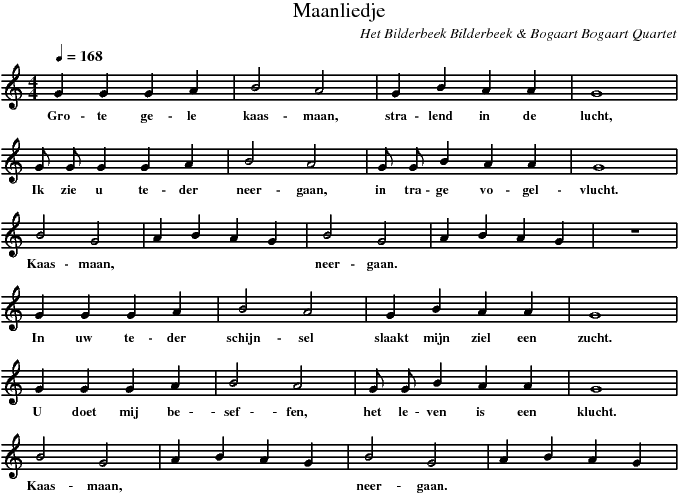
\includegraphics[width=\textwidth,height=\textheight,keepaspectratio]{../songs/01_maanliedje.png}
  \caption{Maanliedje}
  \label{fig:01_maanliedje}
\end{figure}


%%%%%%%%%%%%%%%%%%%%%%%%%%%%%%%%%%%%%%%%%%%%%%%%%%%%%%%%%%%%%%%%%%%%%%%%%%%%%%%%
\section{Grote gele sinaasappel}
%%%%%%%%%%%%%%%%%%%%%%%%%%%%%%%%%%%%%%%%%%%%%%%%%%%%%%%%%%%%%%%%%%%%%%%%%%%%%%%%

\lstinputlisting[
  caption = Grote gele sinaasappel,
  label = lst:02_grote_gele_sinaasappel
]{../songs/02_grote_gele_sinaasappel.txt}

\begin{figure}[!htbp]
  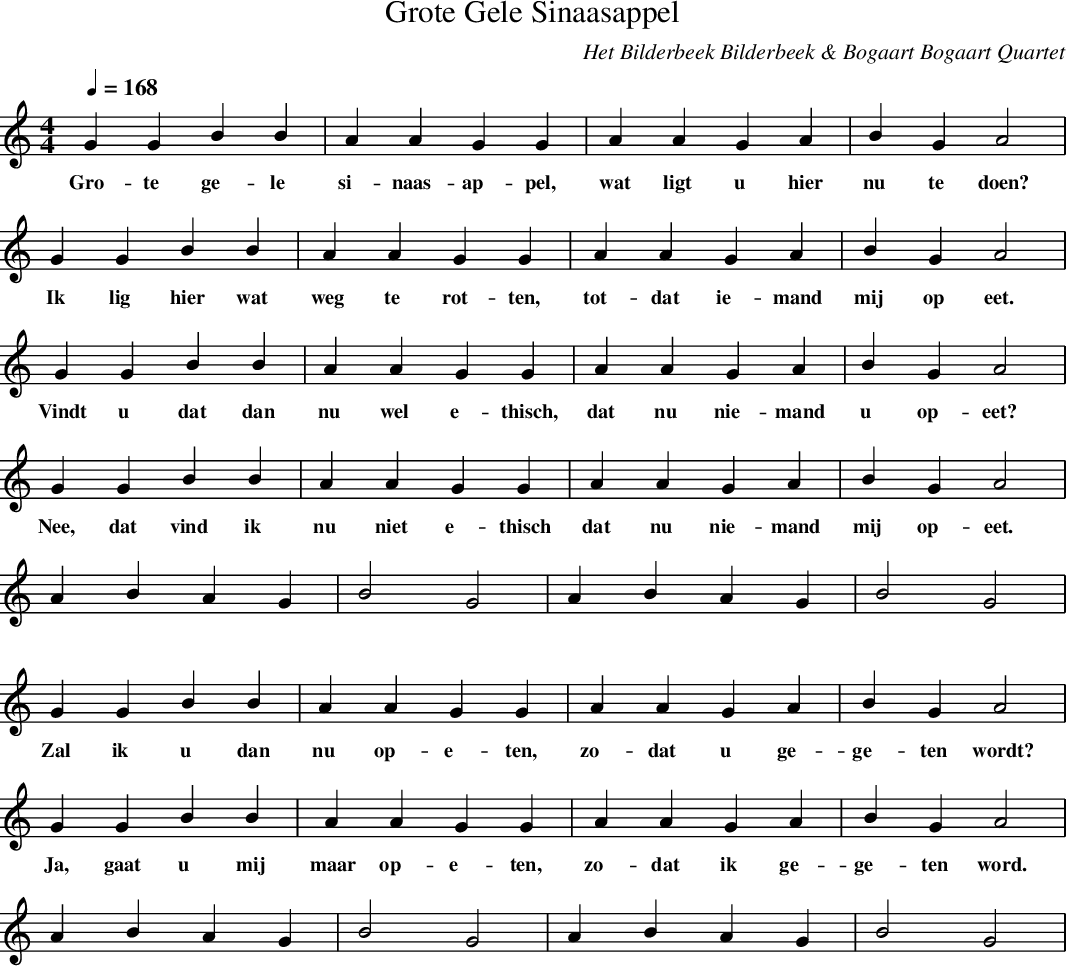
\includegraphics[width=\textwidth,height=\textheight,keepaspectratio]{../songs/02_grote_gele_sinaasappel.png}
  \caption{Grote gele sinaasappel}
  \label{fig:02_grote_gele_sinaasappel}
\end{figure}

%%%%%%%%%%%%%%%%%%%%%%%%%%%%%%%%%%%%%%%%%%%%%%%%%%%%%%%%%%%%%%%%%%%%%%%%%%%%%%%%
\chapter{Ode Aan Masculiniteit}
%%%%%%%%%%%%%%%%%%%%%%%%%%%%%%%%%%%%%%%%%%%%%%%%%%%%%%%%%%%%%%%%%%%%%%%%%%%%%%%%

%\lstinputlisting[
%  caption = Ode Aan Masculiniteit,
%  label = lst:03_ode_aan_masculiniteit
%]{../songs/03_ode_aan_masculiniteit.txt}

\begin{figure}[!htbp]
  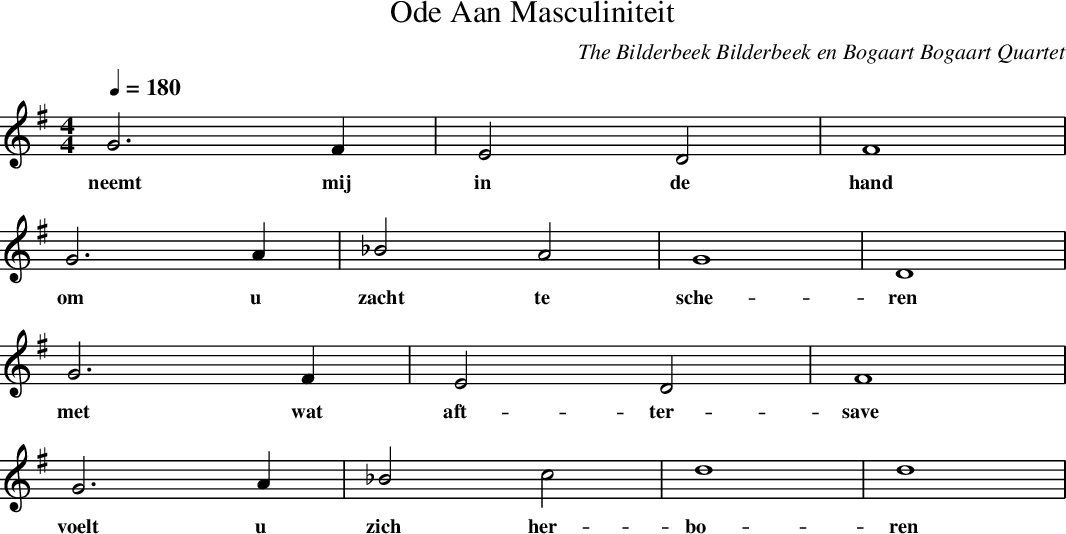
\includegraphics[width=\textwidth,height=\textheight,keepaspectratio]{../songs/03_ode_aan_masculiniteit.png}
  \caption{Ode Aan Masculiniteit}
  \label{fig:03_ode_aan_masculiniteit}
\end{figure}

%%%%%%%%%%%%%%%%%%%%%%%%%%%%%%%%%%%%%%%%%%%%%%%%%%%%%%%%%%%%%%%%%%%%%%%%%%%%%%%%
\section{Het Koffielied}
%%%%%%%%%%%%%%%%%%%%%%%%%%%%%%%%%%%%%%%%%%%%%%%%%%%%%%%%%%%%%%%%%%%%%%%%%%%%%%%%

\lstinputlisting[
  caption = Het Koffielied,
  label = lst:04_het_koffielied
]{../songs/04_het_koffielied.txt}

\begin{figure}[!htbp]
  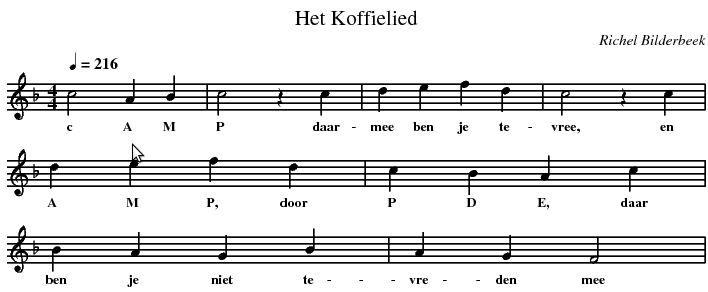
\includegraphics[width=\textwidth,height=\textheight,keepaspectratio]{../songs/04_het_koffielied.png}
  \caption{Het Koffielied}
  \label{fig:04_het_koffielied}
\end{figure}

%%%%%%%%%%%%%%%%%%%%%%%%%%%%%%%%%%%%%%%%%%%%%%%%%%%%%%%%%%%%%%%%%%%%%%%%%%%%%%%%
\section{Hendrik}
%%%%%%%%%%%%%%%%%%%%%%%%%%%%%%%%%%%%%%%%%%%%%%%%%%%%%%%%%%%%%%%%%%%%%%%%%%%%%%%%

\lstinputlisting[
  caption = Hendrik,
  label = lst:05_hendrik
]{../songs/05_hendrik.txt}

\begin{figure}[!htbp]
  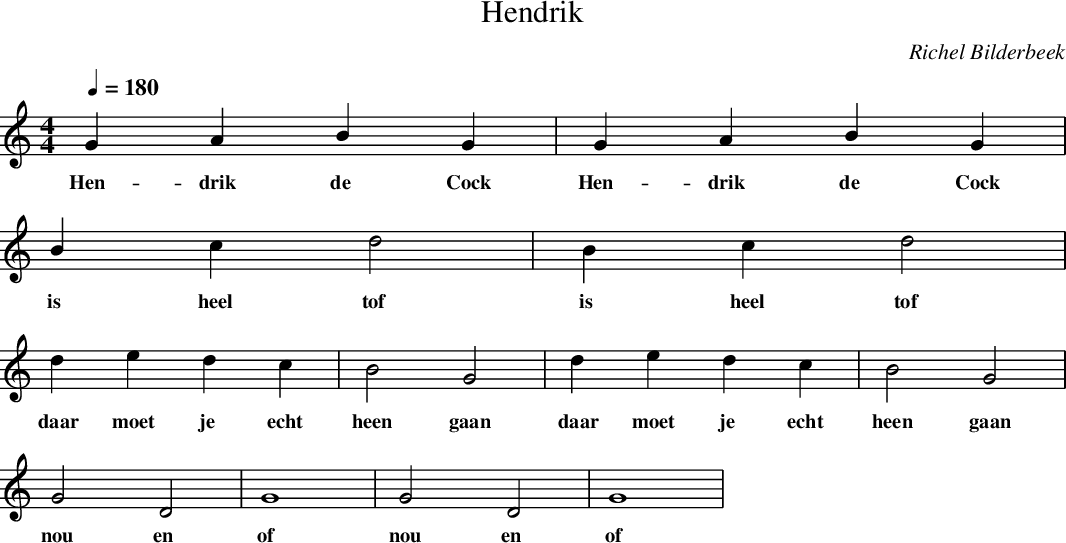
\includegraphics[width=\textwidth,height=\textheight,keepaspectratio]{../songs/05_hendrik.png}
  \caption{Hendrik}
  \label{fig:05_hendrik}
\end{figure}

%%%%%%%%%%%%%%%%%%%%%%%%%%%%%%%%%%%%%%%%%%%%%%%%%%%%%%%%%%%%%%%%%%%%%%%%%%%%%%%%
\section{Leontien}
%%%%%%%%%%%%%%%%%%%%%%%%%%%%%%%%%%%%%%%%%%%%%%%%%%%%%%%%%%%%%%%%%%%%%%%%%%%%%%%%

\lstinputlisting[
  caption = Leontien,
  label = lst:06_leontien
]{../songs/06_leontien.txt}

\begin{figure}[!htbp]
  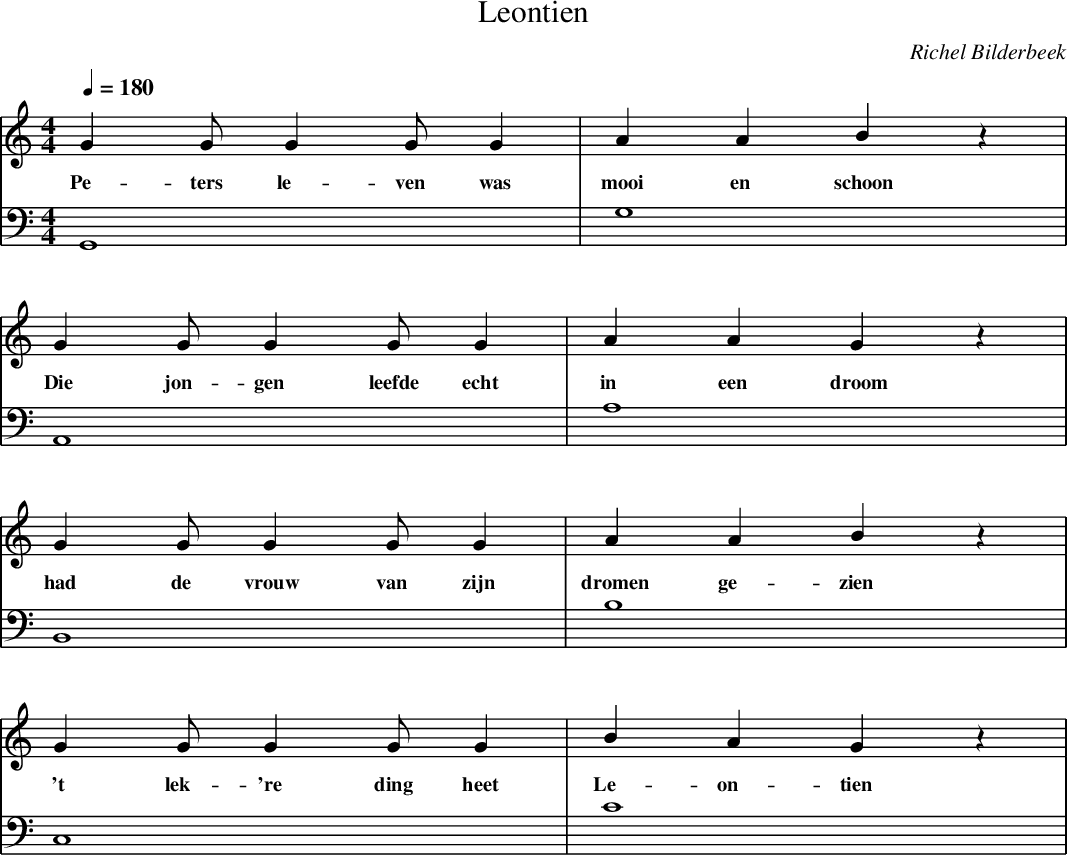
\includegraphics[width=\textwidth,height=\textheight,keepaspectratio]{../songs/06_leontien.png}
  \caption{Leontien}
  \label{fig:06_leontien}
\end{figure}

%%%%%%%%%%%%%%%%%%%%%%%%%%%%%%%%%%%%%%%%%%%%%%%%%%%%%%%%%%%%%%%%%%%%%%%%%%%%%%%%
\chapter{Kinderliefde}
%%%%%%%%%%%%%%%%%%%%%%%%%%%%%%%%%%%%%%%%%%%%%%%%%%%%%%%%%%%%%%%%%%%%%%%%%%%%%%%%

\lstinputlisting[
  caption = Kinderliefde,
  label = lst:07_kinderliefde
]{../songs/07_kinderliefde.txt}

\begin{figure}[!htbp]
  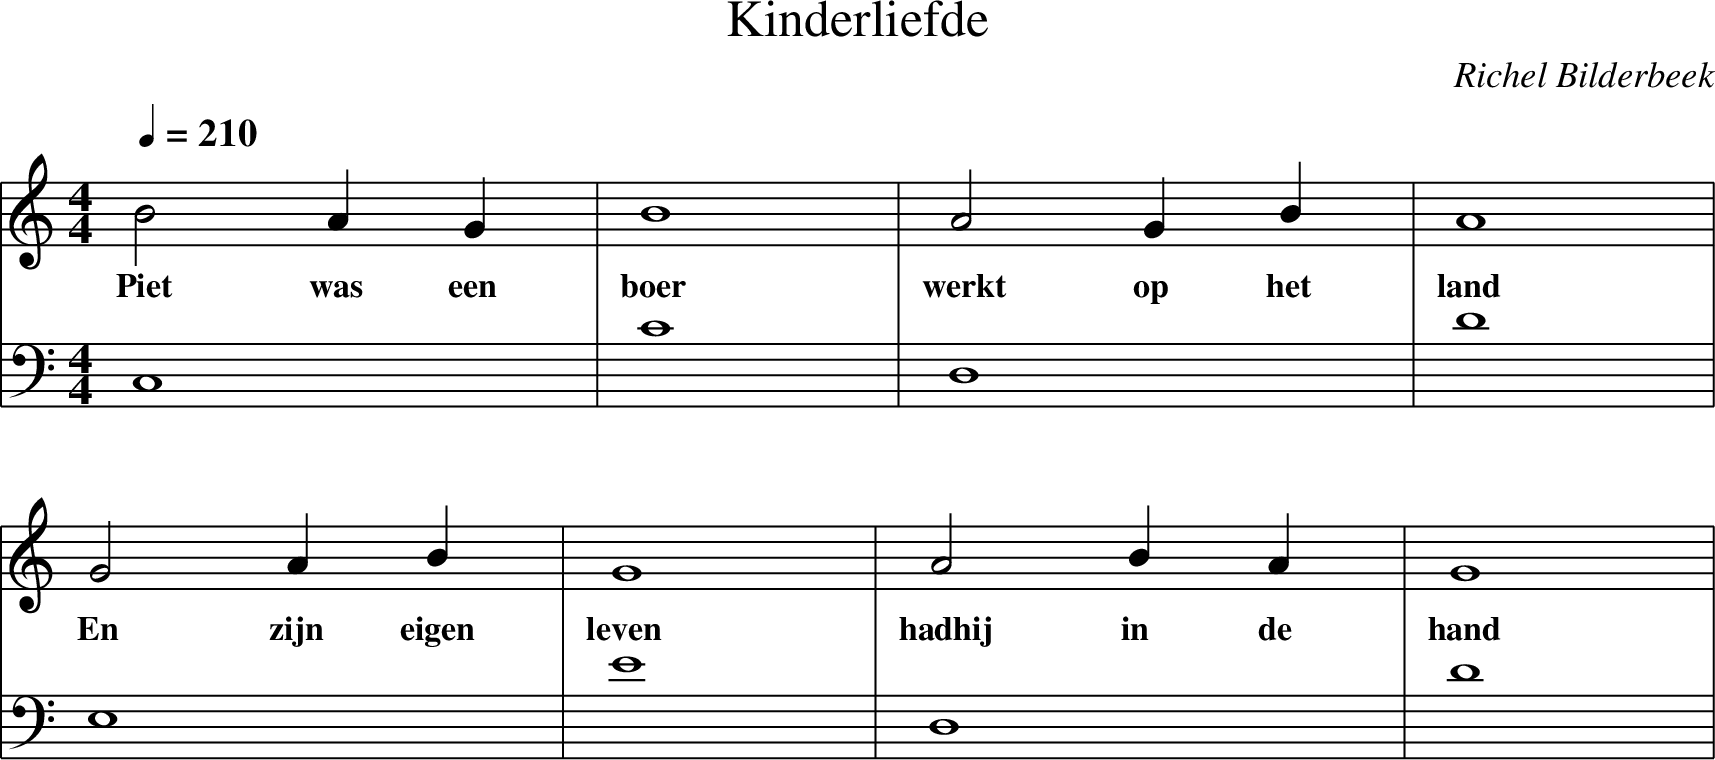
\includegraphics[width=\textwidth,height=\textheight,keepaspectratio]{../songs/07_kinderliefde.png}
  \caption{Kinderliefde}
  \label{fig:07_kinderliefde}
\end{figure}

%%%%%%%%%%%%%%%%%%%%%%%%%%%%%%%%%%%%%%%%%%%%%%%%%%%%%%%%%%%%%%%%%%%%%%%%%%%%%%%%
\chapter{Vroeger}
%%%%%%%%%%%%%%%%%%%%%%%%%%%%%%%%%%%%%%%%%%%%%%%%%%%%%%%%%%%%%%%%%%%%%%%%%%%%%%%%

\lstinputlisting[
  caption = Vroeger,
  label = lst:08_vroeger
]{../songs/08_vroeger.txt}

\begin{figure}[!htbp]
  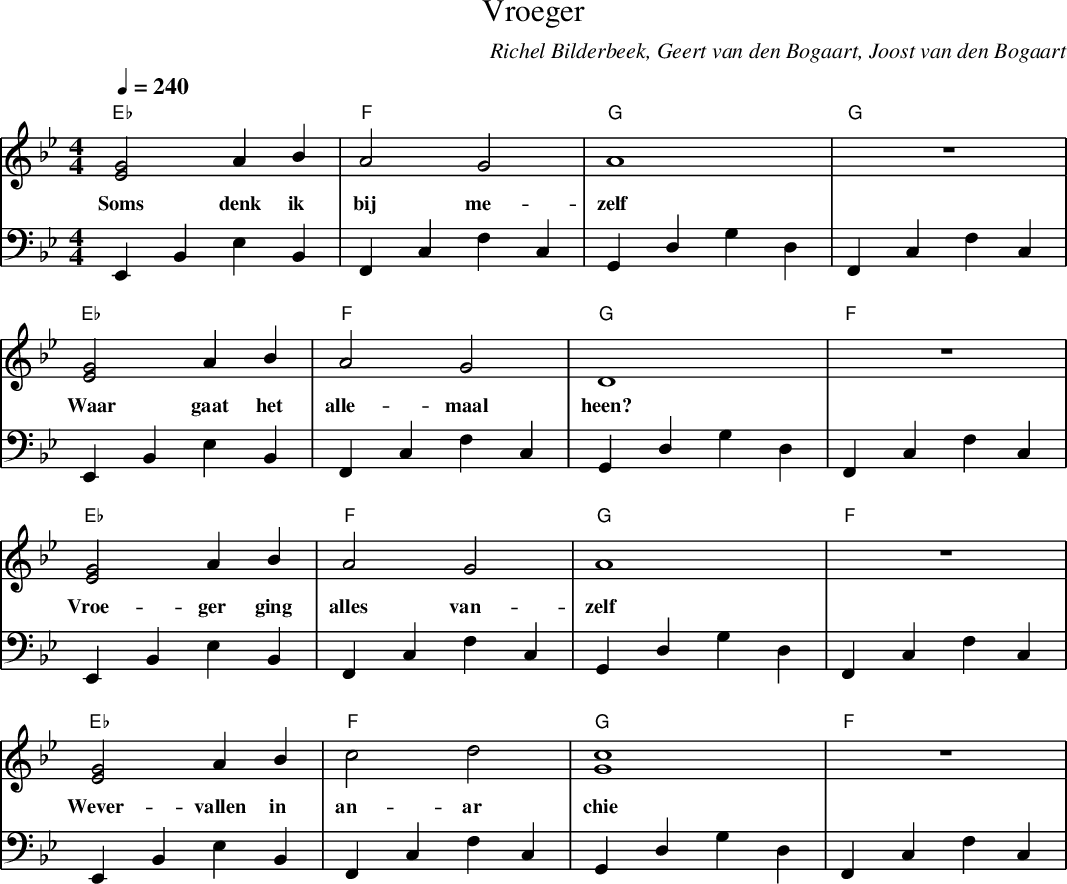
\includegraphics[width=\textwidth,height=\textheight,keepaspectratio]{../songs/08_vroeger.png}
  \caption{Vroeger}
  \label{fig:08_vroeger}
\end{figure}

%%%%%%%%%%%%%%%%%%%%%%%%%%%%%%%%%%%%%%%%%%%%%%%%%%%%%%%%%%%%%%%%%%%%%%%%%%%%%%%%
\chapter{Hendriklied 1}
%%%%%%%%%%%%%%%%%%%%%%%%%%%%%%%%%%%%%%%%%%%%%%%%%%%%%%%%%%%%%%%%%%%%%%%%%%%%%%%%

\lstinputlisting[
  caption = Hendriklied 1,
  label = lst:09_hendriklied_1
]{../songs/09_hendriklied_1.txt}

\begin{figure}[!htbp]
  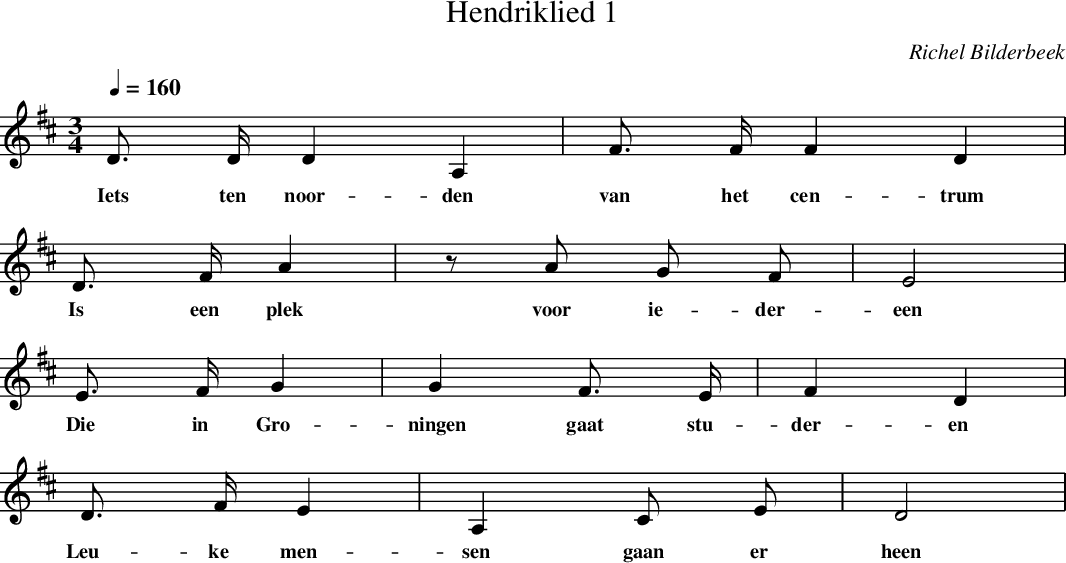
\includegraphics[width=\textwidth,height=\textheight,keepaspectratio]{../songs/09_hendriklied_1.png}
  \caption{Hendriklied 1}
  \label{fig:09_hendriklied_1}
\end{figure}

%%%%%%%%%%%%%%%%%%%%%%%%%%%%%%%%%%%%%%%%%%%%%%%%%%%%%%%%%%%%%%%%%%%%%%%%%%%%%%%%
\section{Hendriklied 2}
%%%%%%%%%%%%%%%%%%%%%%%%%%%%%%%%%%%%%%%%%%%%%%%%%%%%%%%%%%%%%%%%%%%%%%%%%%%%%%%%

\lstinputlisting[
  caption = Hendriklied 2,
  label = lst:10_hendriklied_2
]{../songs/10_hendriklied_2.txt}

%\begin{figure}[!htbp]
%  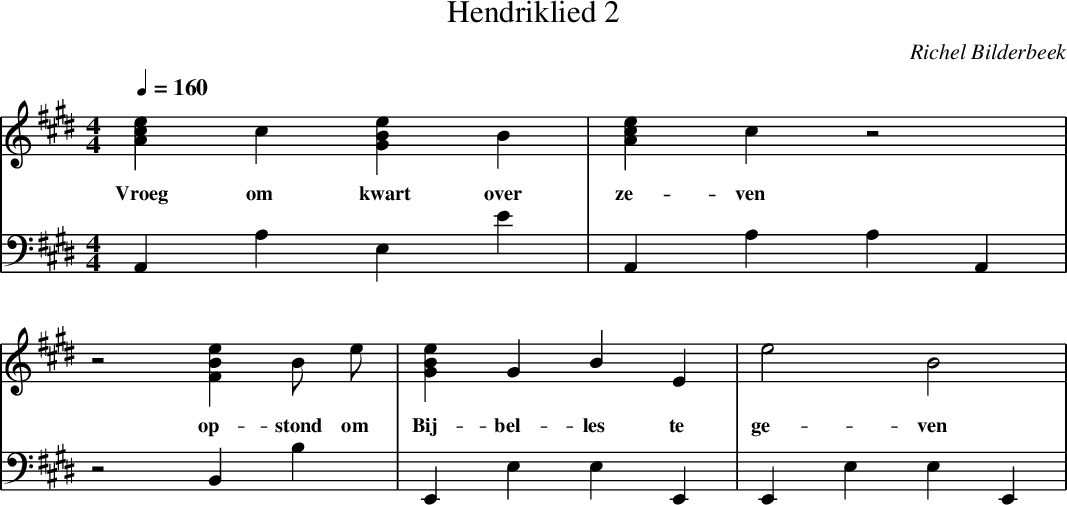
\includegraphics[width=\textwidth,height=\textheight,keepaspectratio]{../songs/10_hendriklied_2.png}
%  \caption{Hendriklied 2}
%  \label{fig:10_hendriklied_2}
%\end{figure}

%%%%%%%%%%%%%%%%%%%%%%%%%%%%%%%%%%%%%%%%%%%%%%%%%%%%%%%%%%%%%%%%%%%%%%%%%%%%%%%%
\section{Rood Geluk}
%%%%%%%%%%%%%%%%%%%%%%%%%%%%%%%%%%%%%%%%%%%%%%%%%%%%%%%%%%%%%%%%%%%%%%%%%%%%%%%%

\lstinputlisting[
  caption = Rood Geluk,
  label = lst:11_rood_geluk
]{../songs/11_rood_geluk.txt}

\begin{figure}[!htbp]
  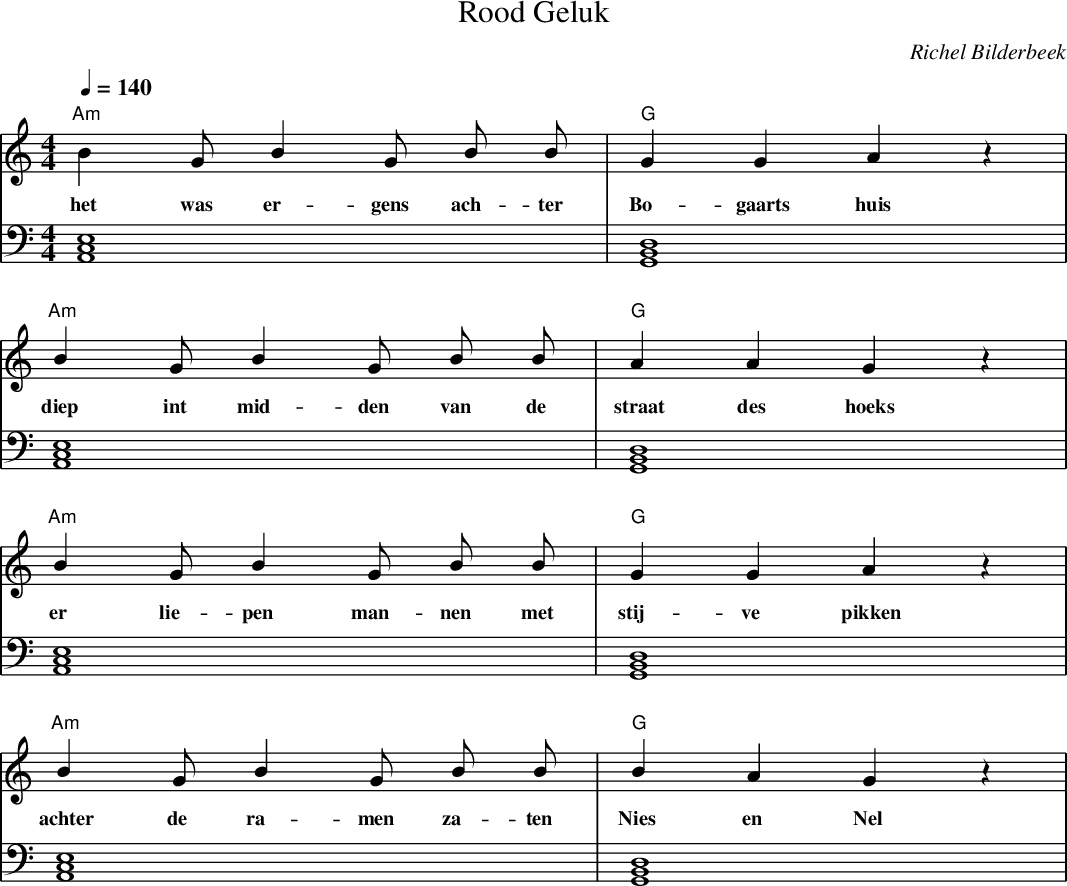
\includegraphics[width=\textwidth,height=\textheight,keepaspectratio]{../songs/11_rood_geluk.png}
  \caption{Rood Geluk}
  \label{fig:11_rood_geluk}
\end{figure}

%%%%%%%%%%%%%%%%%%%%%%%%%%%%%%%%%%%%%%%%%%%%%%%%%%%%%%%%%%%%%%%%%%%%%%%%%%%%%%%%
\section{O, Mooie Geluidsvrouw}
%%%%%%%%%%%%%%%%%%%%%%%%%%%%%%%%%%%%%%%%%%%%%%%%%%%%%%%%%%%%%%%%%%%%%%%%%%%%%%%%

\lstinputlisting[
  caption = O, Mooie Geluidsvrouw,
  label = lst:12_o_mooie_geluidsvrouw
]{../songs/12_o_mooie_geluidsvrouw.txt}

\begin{figure}[!htbp]
  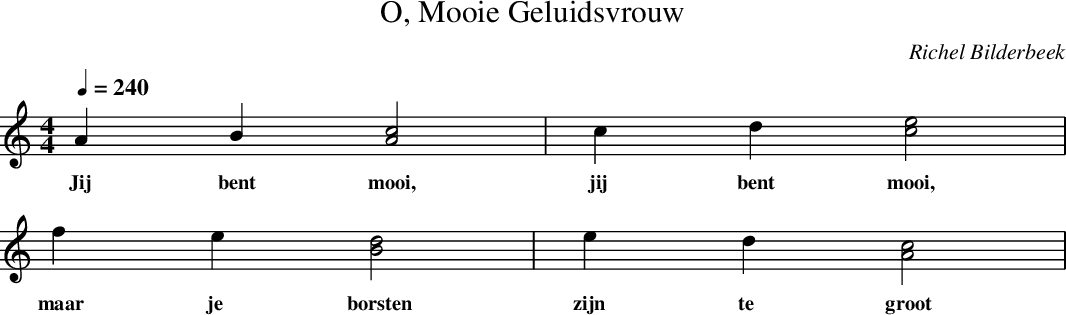
\includegraphics[width=\textwidth,height=\textheight,keepaspectratio]{../songs/12_o_mooie_geluidsvrouw.png}
  \caption{O, Mooie Geluidsvrouw}
  \label{fig:12_o_mooie_geluidsvrouw}
\end{figure}

%%%%%%%%%%%%%%%%%%%%%%%%%%%%%%%%%%%%%%%%%%%%%%%%%%%%%%%%%%%%%%%%%%%%%%%%%%%%%%%%
\section{Hendriklied 3}
%%%%%%%%%%%%%%%%%%%%%%%%%%%%%%%%%%%%%%%%%%%%%%%%%%%%%%%%%%%%%%%%%%%%%%%%%%%%%%%%

\lstinputlisting[
  caption = Hendriklied 3,
  label = lst:13_hendriklied_3
]{../songs/13_hendriklied_3.txt}

\begin{figure}[!htbp]
  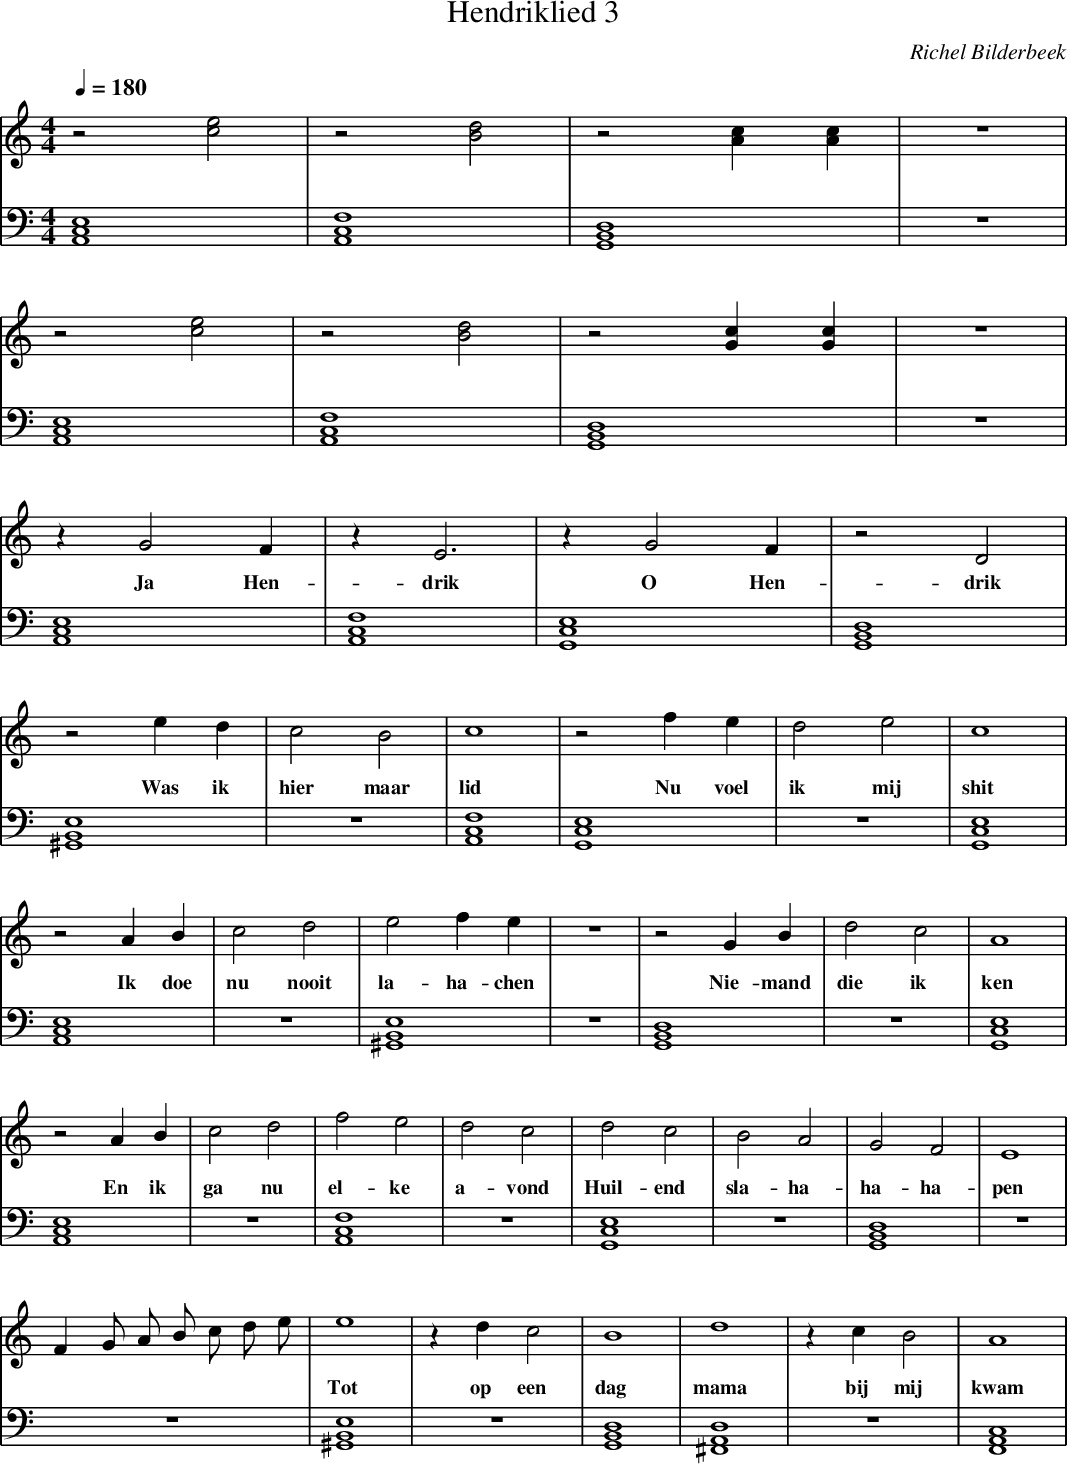
\includegraphics[width=\textwidth,height=\textheight,keepaspectratio]{../songs/13_hendriklied_3-0.png}
  \caption{Hendriklied 3 1/2}
  \label{fig:13_hendriklied_3_1}
\end{figure}

\begin{figure}[!htbp]
  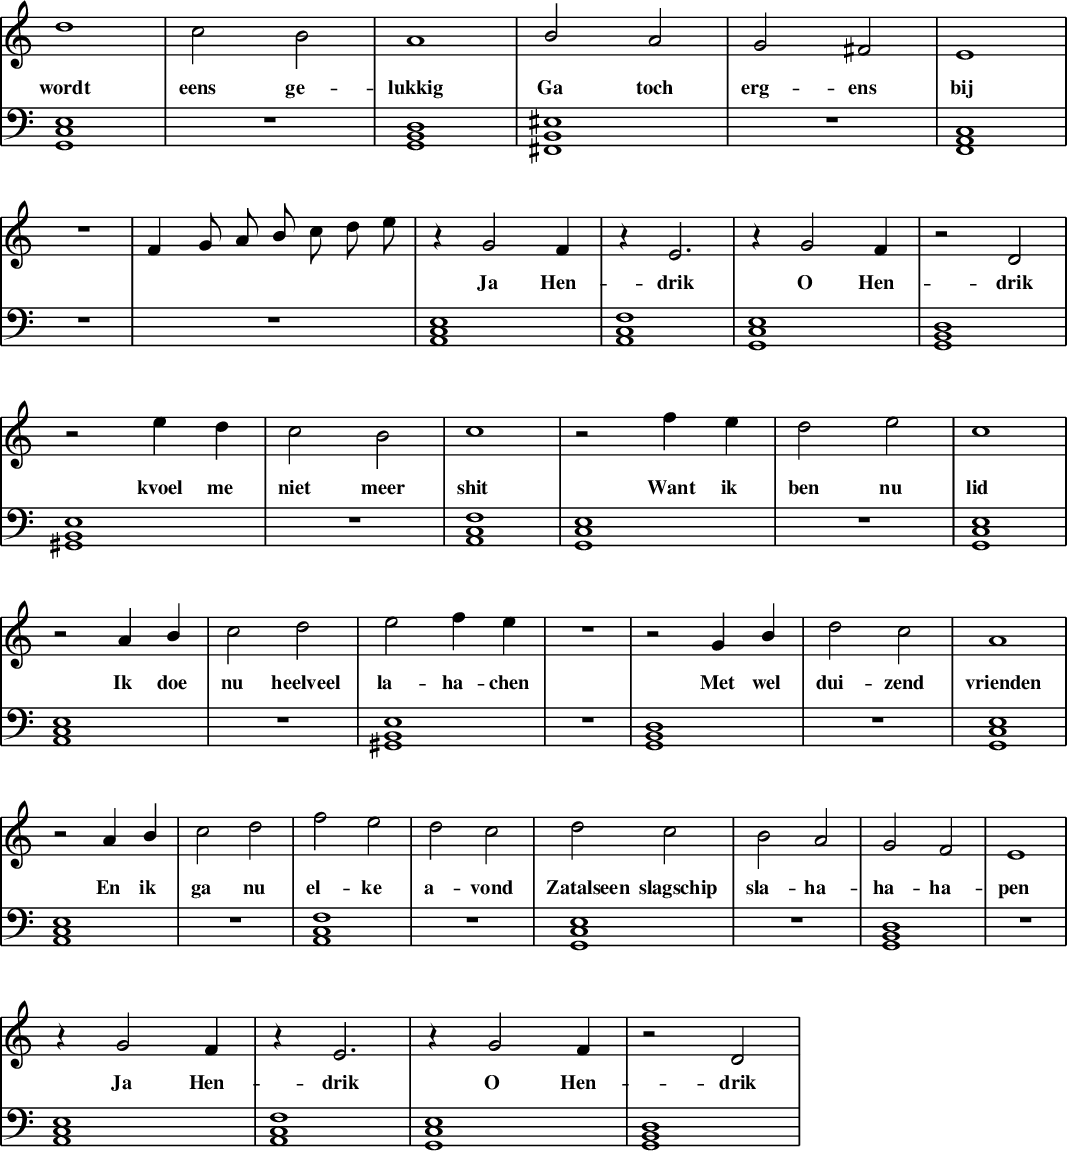
\includegraphics[width=\textwidth,height=\textheight,keepaspectratio]{../songs/13_hendriklied_3-1.png}
  \caption{Hendriklied 3 2/2}
  \label{fig:13_hendriklied_3_2}
\end{figure}

%%%%%%%%%%%%%%%%%%%%%%%%%%%%%%%%%%%%%%%%%%%%%%%%%%%%%%%%%%%%%%%%%%%%%%%%%%%%%%%%
\section{Come Home Darling}
%%%%%%%%%%%%%%%%%%%%%%%%%%%%%%%%%%%%%%%%%%%%%%%%%%%%%%%%%%%%%%%%%%%%%%%%%%%%%%%%

\lstinputlisting[
  caption = Come Home Darling,
  label = lst:14_come_home_darling
]{../songs/14_come_home_darling.txt}

\begin{figure}[!htbp]
  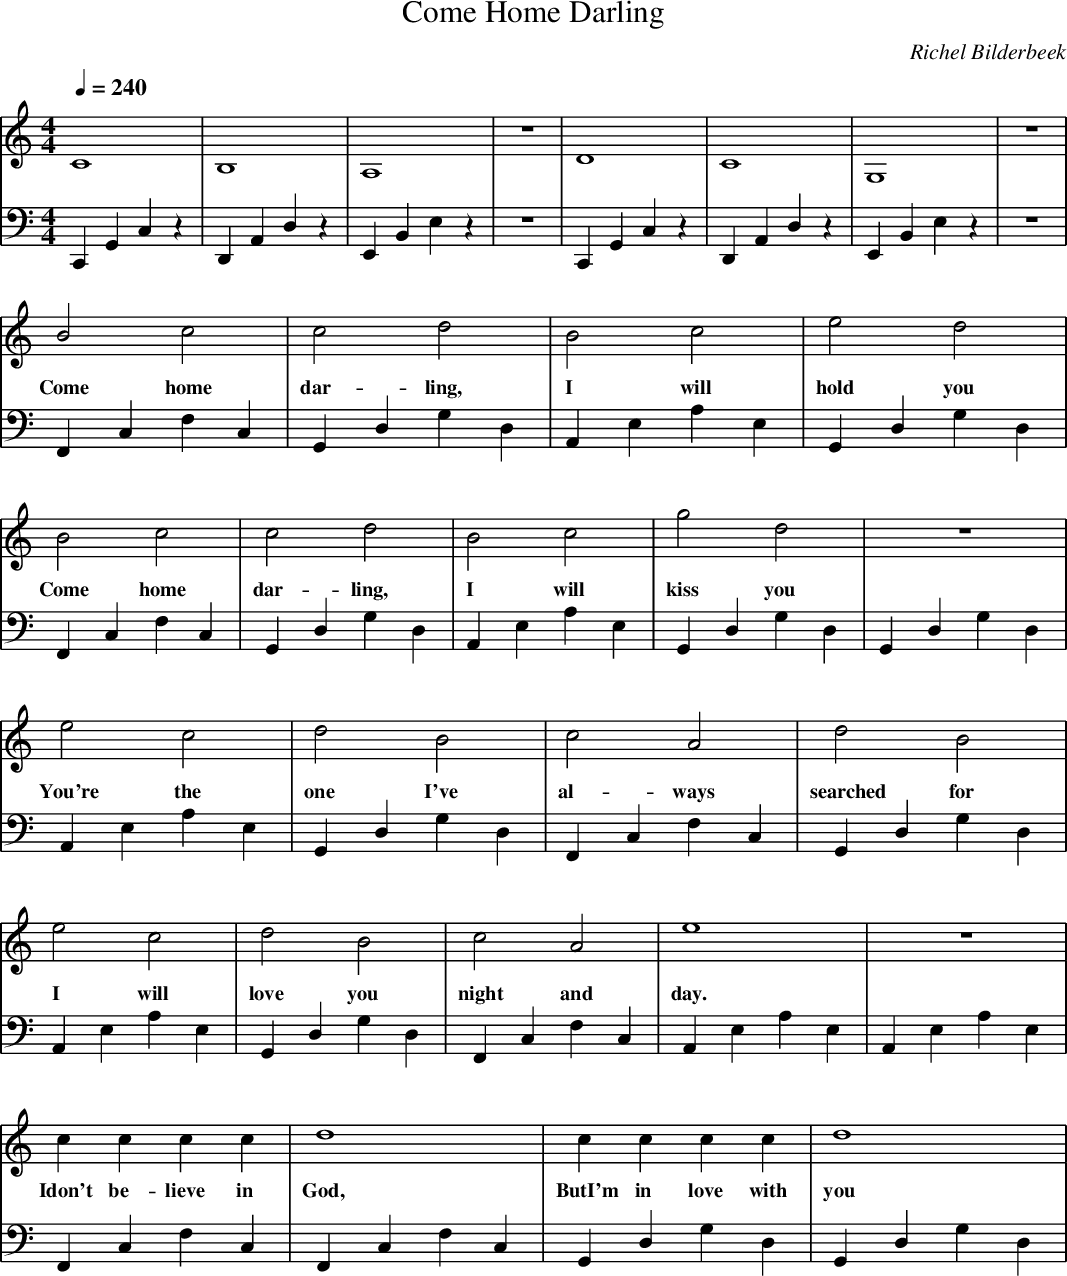
\includegraphics[width=\textwidth,height=\textheight,keepaspectratio]{../songs/14_come_home_darling-0.png}
  \caption{Come Home Darling 1/2}
  \label{fig:14_come_home_darling_1}
\end{figure}

\begin{figure}[!htbp]
  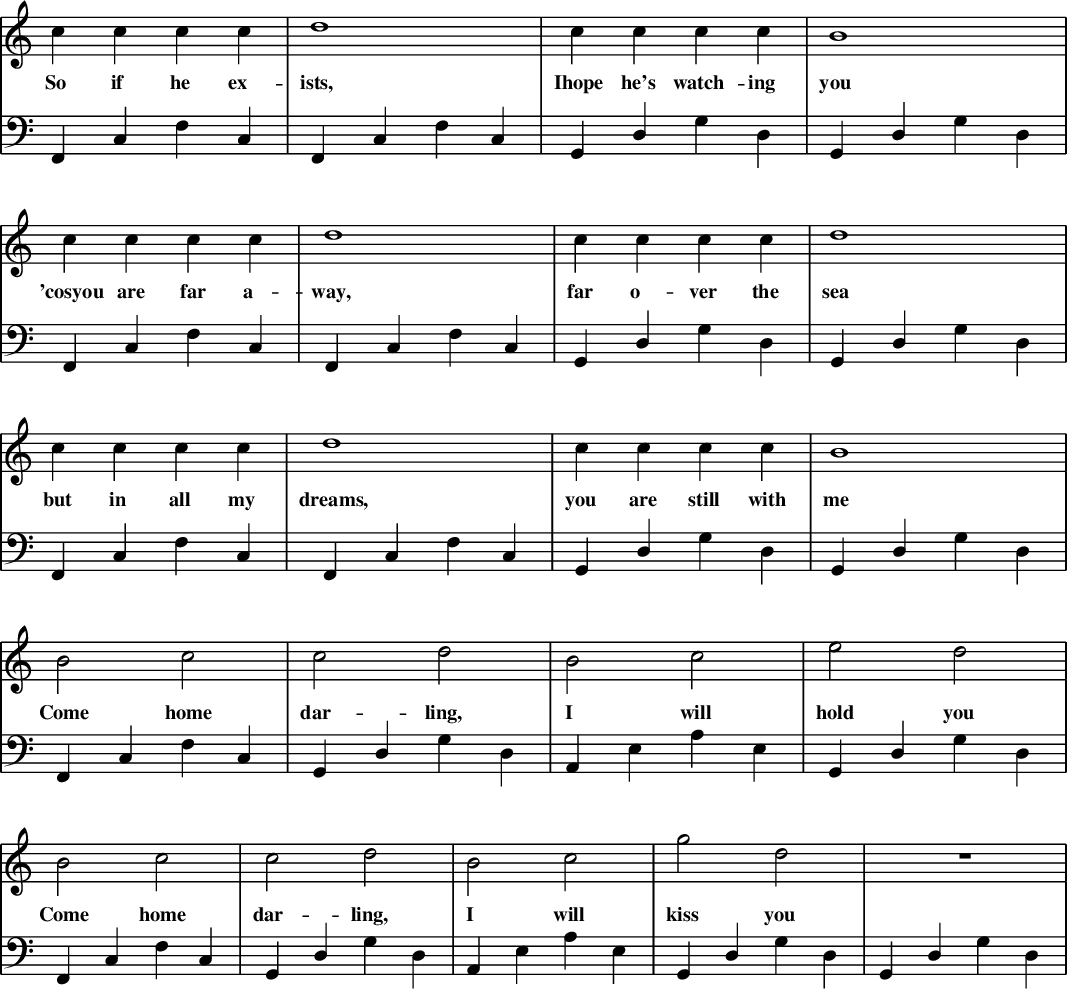
\includegraphics[width=\textwidth,height=\textheight,keepaspectratio]{../songs/14_come_home_darling-1.png}
  \caption{Come Home Darling 2/2}
  \label{fig:14_come_home_darling_2}
\end{figure}

%%%%%%%%%%%%%%%%%%%%%%%%%%%%%%%%%%%%%%%%%%%%%%%%%%%%%%%%%%%%%%%%%%%%%%%%%%%%%%%%
\section{Het Neukmenslied}
%%%%%%%%%%%%%%%%%%%%%%%%%%%%%%%%%%%%%%%%%%%%%%%%%%%%%%%%%%%%%%%%%%%%%%%%%%%%%%%%

\lstinputlisting[
  caption = Het Neukmenslied,
  label = lst:15_het_neukmenslied
]{../songs/15_het_neukmenslied.txt}

\begin{figure}[!htbp]
  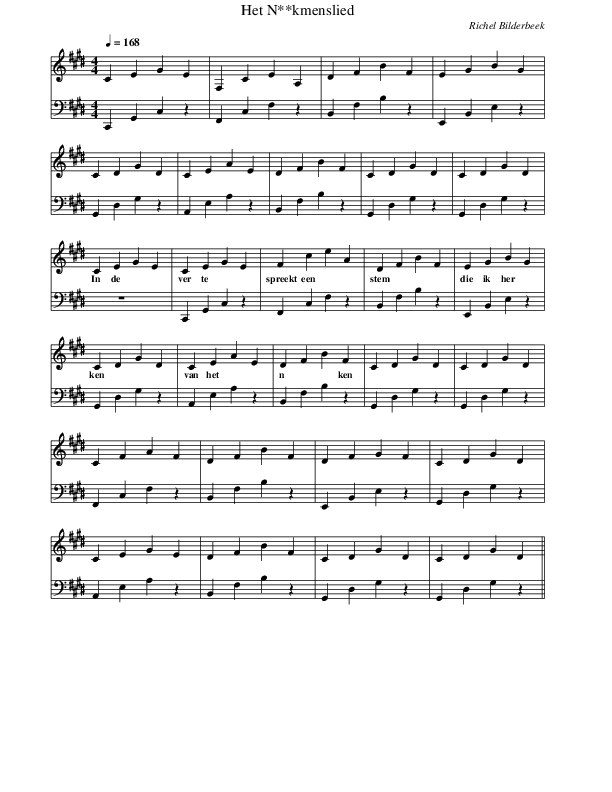
\includegraphics[width=\textwidth,height=\textheight,keepaspectratio]{../songs/15_het_neukmenslied.png}
  \caption{Het Neukmenslied}
  \label{fig:15_het_neukmenslied}
\end{figure}

%%%%%%%%%%%%%%%%%%%%%%%%%%%%%%%%%%%%%%%%%%%%%%%%%%%%%%%%%%%%%%%%%%%%%%%%%%%%%%%%
\section{Het Mentorkindjeslied}
%%%%%%%%%%%%%%%%%%%%%%%%%%%%%%%%%%%%%%%%%%%%%%%%%%%%%%%%%%%%%%%%%%%%%%%%%%%%%%%%

\lstinputlisting[
  caption = Het Mentorkindjeslied,
  label = lst:16_het_mentorkindjeslied
]{../songs/16_het_mentorkindjeslied.txt}

\begin{figure}[!htbp]
  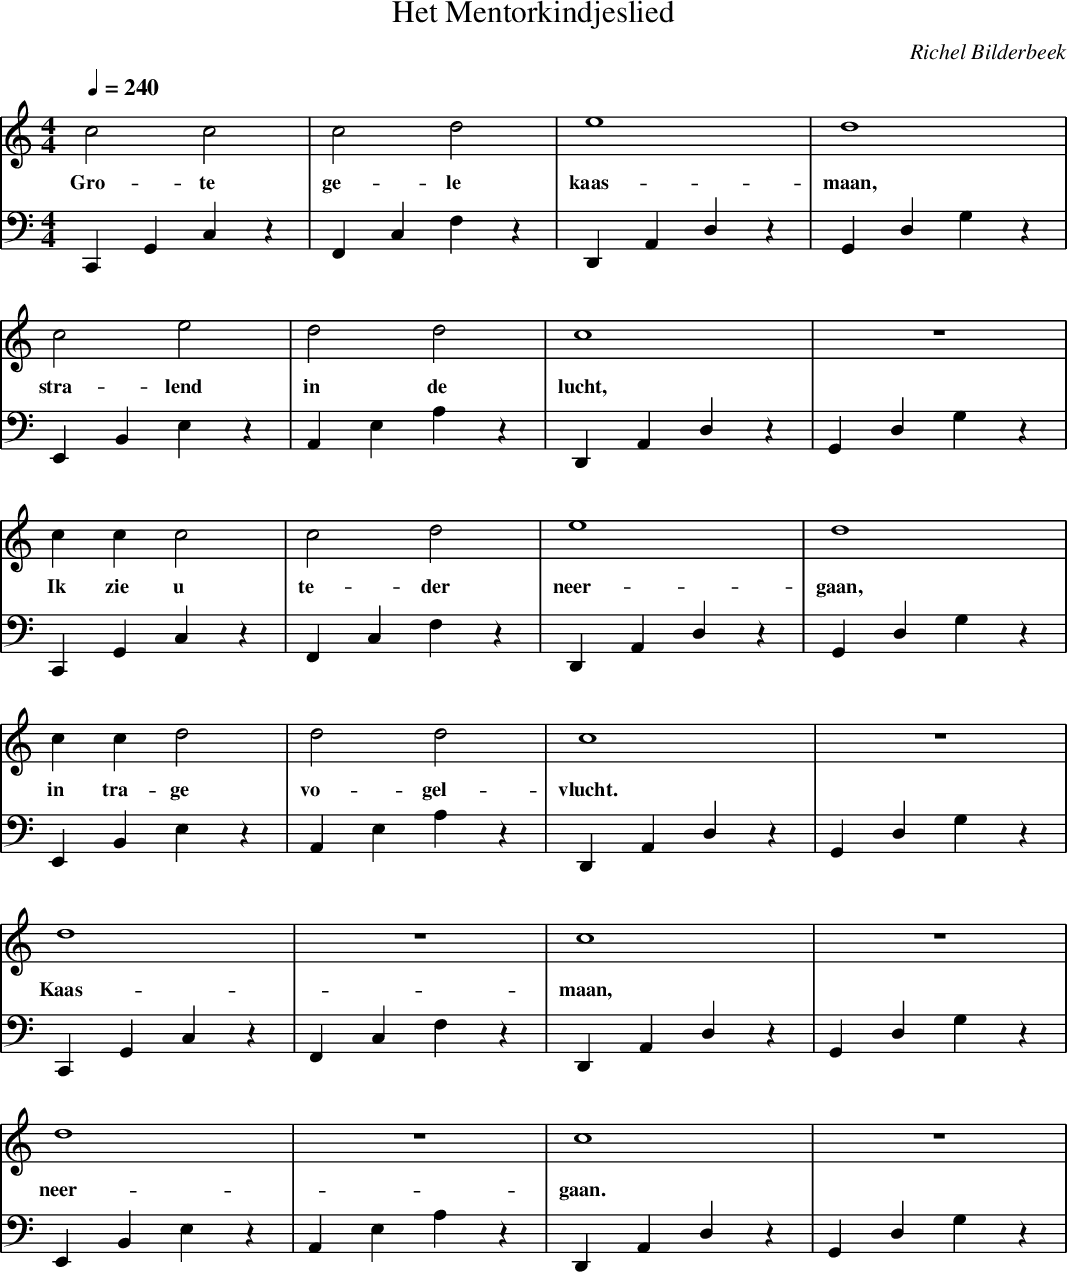
\includegraphics[width=\textwidth,height=\textheight,keepaspectratio]{../songs/16_het_mentorkindjeslied.png}
  \caption{Het Mentorkindjeslied}
  \label{fig:16_het_mentorkindjeslied}
\end{figure}


% 16 | 2002-09-14 | [Het Mentorkindjeslied](HetMentorkindjeslied.md)
% 17 | 2002-10-05 | [Hoggamus Higgamus](HoggamusHiggamus.md)
% 18 | 2002-12-19 | [Het Leven Is Naar](HetLevenIsNaar.md)
% 19 | 2003-??-?? | [Het Leven Is Een ..... .............](HetLevenIsEenVuileKolerelijer.md)
% 20 | 2003-04-05 | [Al Heb Je Blauw Haar](AlHebJeBlauwHaar.md)
% 21 | 2003-08-12 | [Wooloo Mooloo](WoolooMooloo.md)
% 22 | 2003-12-01 | [Mannen](Mannen.md)
% 23 | 2004-01-18 | [Slaapliedje](Slaapliedje.md)
% 24 | 2004-02-12 | [De ...](DeLul.md)
% 25 | 2004-03-07 | [Blauw](Blauw.md)
% 26 | 2004-06-03 | [Morgenvroeg](Morgenvroeg.md)
% 27 | 2004-06-07 | [Zonder Jou Weg](ZonderJouWeg.md)
% 28 | 2004-11-02 | [Klavierstueckchen](Klavierstueckchen.md)
% 29 | 2004-11-25 | [Dortmund](Dortmund.md)
% 30 | 2005-01-29 | [Die Rolltreppe Und Ich](DieRolltreppeUndIch.md)
% 31 | 2005-??-?? | [Blau](Blau.md)
% 32 | 2005-??-?? | [Kaesemond](Kaesemond.md)
% 33 | 2005-??-?? | [Wooloo Mooloo (DE)](WoolooMoolooDe.md)
% 34 | 2005-??-?? | [Morgensfrueh](Morgensfrueh.md)
% 35 | 2005-??-?? | [Wenn Du Haettest Blaue Haare](WennDuHaettestBlaueHaare.md)
% 36 | 2005-??-?? | [Der .......](DerSchwanz.md)
% 37 | 2005-??-?? | [Das ....menslied](DasFickmenschlied.md)
% 38 | 2005-??-?? | [Das Leben ist ....](DasLebenIstMist.md)
% 39 | 2005-??-?? | [Das Kaffeelied](DasKaffeelied.md)
% 40 | 2005-05-24 | [The Clifton Suspension Bridge](TheCliftonSuspensionBridge.md)
% 41 | 2005-06-04 | [You And Me](YouAndMe.md)
% 42 | 2005-07-07 | [To The Pub](ToThePub.md)
% 43 | 2005-??-?? | [Even If Your Hair Is Blue](EvenIfYourHairIsBlue.md)
% 44 | 2005-??-?? | [Life Is A .....](LifeIsAbitch.md)
% 45 | 2005-10-15 | [Plank OpWieltjes](PlankOpWieltjes.md)
% 46 | 2005-10-22 | [Koud Bloed In Mijn Hart](KoudBloedInMijnHart.md)
% 47 | 2005-11-15 | [Mijn Date Van Vrijdagavond](MijnDateVanVrijdagavond.md)
% 48 | 2006-05-20 | [Achter Mijn Raam](AchterMijnRaam.md)
% 49 | 2007-01-28 | [Ben Ik Een Spin](BenIkEenSpin.md)
% 50 | 2007-09-29 | [Organellenwals](Organellenwals.md)
% 51 | 2007-09-29 | [Stuk eiwit](StukEiwit.md)
% 52 | 2009-10-30 | [Heejaa Mama](HeejaaMama.md)
% 53 | 2010-11-10 | [Voor De Klas](VoorDeKlas.md)
% 54 | 2011-04-07 | ["Friday"](Friday.md)
% 55 | 2011-04-24 | [Vrouwen Van JeDromen](VrouwenVanJeDromen.md)
% 56 | 2012-08-04 | [Groningen Danst](GroningenDanst.md)
% 57 | 2013-06-20 | [Superman B](SupermanB.md)
% 58 | 2013-06-21 | [Hee Ga Je Mee](HeeGaJeMee.md)
% 59 | 2013-06-26 | [Een](Een.md)
% 60 | 2014-01-15 | [Liefdeskapitein](Liefdeskapitein.md)
% 61 | 2014-02-14 | [Mars](Mars.md)
% 62 | 2015-02-15 | [Pjanoman](Pjanoman.md)
% 63 | 2018-02-07 | [Monsieur Pannetier](MonsieurPannetier.md)
% 64 | 2018-03-03 | [16777216 Kleuren](16777216Kleuren.md)
% 


\end{document}
